\section{\label{sec:results}Results from Optical Pumping Cell Geometries}
\begin{figure*}
    \subfloat[The 100 cc horizontal geometry with a full-circumferential shell for the Rb source.\label{fig:fullcell}]{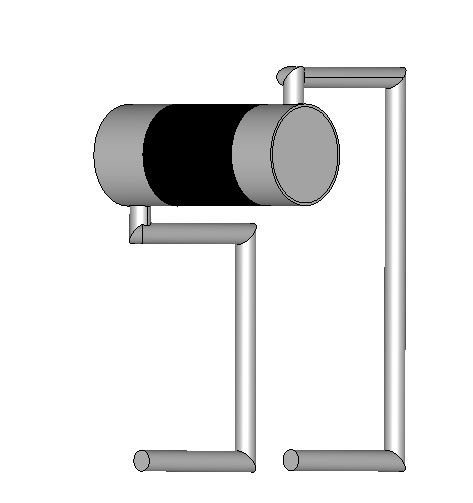
\includegraphics[width=0.33\textwidth]{Figures/RbGeometry.png}}
    \subfloat[The 100 cc vertical geometry with a full-circumferential shell for the Rb source.\label{fig:fullcellvert}]{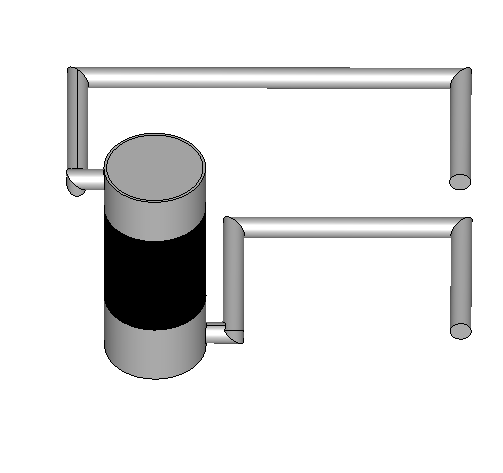
\includegraphics[width=0.33\textwidth]{Figures/RbGeometryVert.png}}\\
    \subfloat[The 100 cc horizontal geometry with a half-circumferential shell for the Rb source. This was also modelled in a vertical orientation like the geometry in Figure \ref{fig:fullcellvert}.\label{fig:halfcell}]{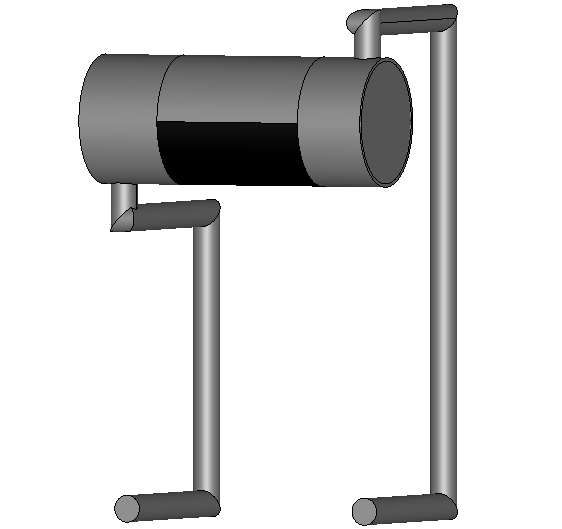
\includegraphics[width=0.33\textwidth]{Figures/100cchalf.png}}
    \subfloat[The 300 cc horizontal geometry with a drop for the Rb source.\label{fig:rbdropcell}]{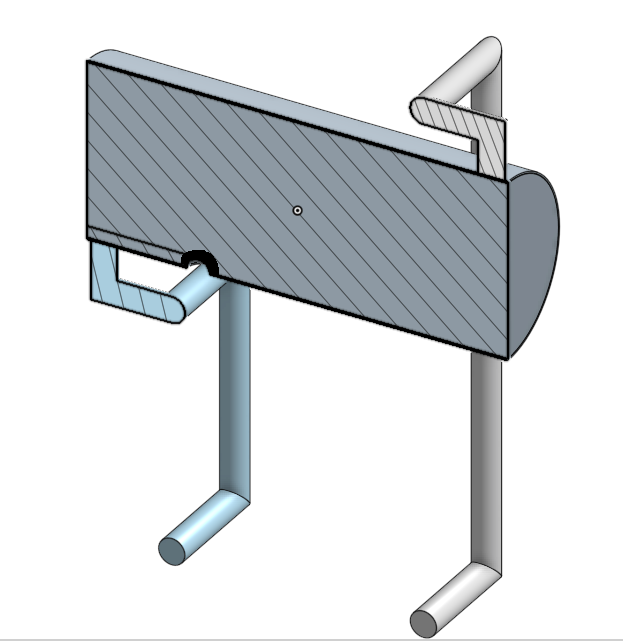
\includegraphics[width=0.33\textwidth]{Figures/RbDrop.png}}
    \caption{The different geometries that were modelled in the current study. The 100 cc optical cells were model with a full-circumferential shell (\ref{fig:fullcell} and \ref{fig:fullcellvert}) and a half-circumferential shell (\ref{fig:halfcell}). A 300 cc optical pumping cell was also modelled with a Rb drop for an in-body source (\ref{fig:rbdropcell}). Visualization of the different optical pumping cell geometries used in the The geometries were modelled with a constant gravitational body force, and two orientation were used: horizontal (\ref{fig:fullcell}, \ref{fig:halfcell}, and \ref{fig:rbdropcell}) and vertical (\ref{fig:fullcellvert}, half-circumferential vertical cell not shown). In the figures, areas in black represent the in-body Rb sources. The outlet sources are not pictured in the figures.}
    \label{fig:allgeometries}
\end{figure*}
\begin{table*}[t]
\caption{Results of 100 cc simulations at all temperatures. The top row describes the four different Rb configuration and cell orientation combinations used in the simulations. The results are described in four ways: (1) full oscillations were observed, (2) possible oscillations were observed, (3) a rapid rise in temperature and laser absorption were observed, and (4) a steady-state solution was observed. Text in italics denotes that premature termination of the simulation resulted in low fidelity data that made firm conclusions difficult.\label{tab:all100ccresults}}
\begin{tabular}{c|c|c?c|c|}
    &\textbf{Full-Horz.}    &\textbf{Full-Vert.}    &\textbf{Half-Horz.}         & \textbf{Half-Vert.}\\ \hline
\textbf{110 $^{\circ}$C}& Steady-State  & Steady-State  & Steady-State       & Steady-State \\ \hline
\textbf{120 $^{\circ}$C}& Full Osc.     & Full Osc.     & \textit{Rapid Temp. and Abs. Increase} & Full Osc. \\ \hline
\textbf{130 $^{\circ}$C}& Full Osc.      & Full Osc.    & \textit{Possible Osc.} &\textit{Possible Osc.} \\ \hline
\textbf{140 $^{\circ}$C}& \textit{Possible Osc.}\ & Full Osc.    & \textit{Possible Osc.} &\textit{Possible Osc.}\\ \hline
\end{tabular}
\end{table*}
In the section \ref{sec:verification}, the FEM model was applied to a cylindrical geometry. A more interesting case is applying the model to a geometry which approximates a standard optical pumping cell. Three different geometries where investigated in the course of this study: (1) a 100 cc cell with a full circumferential Rb distribution, (2) a 100 cc cell with a half-circumferential Rb distribution, and a 300 cc cell with a Rb drop (see Figure \ref{fig:allgeometries}).

Rb sources for the diffusion module were modelled in two areas in the optical pumping cell geometries. First, a Rb source was modelled in the optical pumping body (cylindrical portion). This source was either modelled as a thin film (100 cc cells, e.g. Figure \ref{fig:fullcell}) or a drop (300 cc cell, e.g. Figure \ref{fig:rbdropcell}).

The second source/sink was modelled as a thin film in the outlet of the cell. In the 100 cc cells, this thin film started at the joint between the outlet and the cell body, and it extended to the final bend in the outlet. Two different configurations were used for the Rb source in the outlet of the 300 cc cell: (1) the same configuration as the 100 cc cells, and (2) the thin film started at the first bend in the outlet and extended to the final bend in the outlet.  

A body force was applied in the Navier-Stokes module to simulate gravity and enable gas convection in the simulation. This force was oriented either such that the cell was oriented horizontally (e.g. Figure \ref{fig:fullcell}) or vertically (e.g. Figure \ref{fig:fullcellvert}). The vertical case was only investigated in the 100 cc cells.

Cells were modelled at four wall-temperature boundary conditions: 110 $^{\circ}$C, 120 $^{\circ}$C, 130 $^{\circ}$C, 140 $^{\circ}$C. These different boundary conditions simulated different oven-air temperatures that the optical pumping cell could experience. These temperatures were the values assigned to $T_{ext}$ from eq. \ref{eq:tempboundary}. 

Results for the 100 cc-cell simulations are shown in Table \ref{tab:all100ccresults}, and three sample visualizations of the results are shown in Figure \ref{fig:resultvisualization}. The models in most cases did not reach a steady-state solution. Many of the simulations displayed a strong oscillatory behavior in average temperature, Rb polarization, and laser absorption. Other simulations displayed possible oscillatory behavior. However, difficulties with model convergence caused the simulation to terminate prematurely and in some cases, affected the model's behavior. These premature terminations made it difficult to come to firm conclusions on the long-term behavior of the model for those parameters. Finally, one 100 cc model reached neither steady-state nor displayed oscillatory behavior, but instead displayed a rapid rise in average temperature and laser absorption before terminating prematurely. Again, the premature termination makes it difficult to predict the long-term behavior of the model at these parameters.

The oscillatory cycles followed a common pattern. During the initial stage, the Rb polarization remained high and stable, but the average cell temperature and laser absorption steadily rose. This state remained until the average gas temperature was roughly 100\% higher than wall boundary condition temperature. At this point, the Rb polarization rapidly decreased, while the laser absorption and temperature rapidly increased. 

This sudden change was accompanied by a marked change in the gas flow behavior. In the horizontally oriented cells, the convection rotation changed orientations from rotating about the axis of the cell body cylinder to rotating in the about an axis in the transverse plane. Cells oriented vertically show a tightening of the convection rotation towards the front of the cell. In the case of horizontal cells, this new flow pattern remains even after the average temperature had decreased. In vertical cells, the flow pattern oscillated with the average temperature and laser absorption. 

The average temperature in the cells peak at $\approx$150\% of the wall boundary condition, and the Rb polarization falls to $\approx$ 0\%. At this point, the Rb vapor has absorbed most of the laser light at the front of the cell. This allowed the temperature of the gas in most of the cell to fall rapidly. As the average temperature decreased, both the Rb vapor number density and laser absorption decreased allowing the laser to, once again, penetrate deep into the optical pumping cell.

In addition to this oscillatory behavior, the models predicted points in the cell whose temperature exceed 1000 $^{\circ}$C, which is very likely a non-physical result. If this configuration of Rb is ever realized in an optical pumping cell, the Rb film experiencing high temperatures is likely to relocate to another portion of the cell. The Rb sources in the FEMt model are inexhaustible and static.

The 300 cc optical pumping cell model was constructed after completing the initial simulations with the 100 cc models. The model's construction attempted to eliminate the above described oscillatory behavior, as it is not observed in experimental setups. First, the volume of the cell was increased to decrease the modelled intensity of the laser beam and decrease the likelihood of generating non-physical temperatures. In addition, the Rb source in the the body of the cell was reconfigured to a single drop structure on the bottom surface of the optical pumping cell body. Initially, a Rb sink in the form of a thin film on the walls of the outlet was maintained as in the 100 cc cells. The cell was only simulated in the horizontal orientation. The results are shown in Table \ref{tab:all300ccresults}, and samples of visualization are shown in Figures \ref{fig:300ccrboutletresult} and \ref{fig:results300ccresult}. 

In the initial simulation of this configuration (Figure \ref{fig:300ccrboutletresult}), the model again predicted that the gasses in the body of the cell are heated. Due to the configuration and cell dimensions, the temperature near the Rb drop does not significantly rise. However, the gasses exiting through the outlet can be several hundred degrees above the set point temperature.

Excessive heating of the Rb source/sink in the outlet caused an excess of Rb vapor. Due to the proximity of the modelled source to the cell body, some of this excess was able to diffuse back into the cell body and block substantial portions of the light. Eventually, the Rb source in the outlet became the dominate source of Rb vapor in the body of the cell, and the laser adsorption dramatically increased. The simulation terminated prematurely, so it is unclear if this system would generate oscillations as observed in the 100 cc cells.

A second 300 cc geometry was generated with the outlet Rb source/sink recessed farther into the outlet in order to prevent the vapors from this source diffusing back into the body of the cell. The outlet Rb source/sink in this model started at the first bend in the outlet. In this configuration, the hot exit gasses again heated the Rb in the outlet and generated excess Rb. However, because the Rb film was recessed farther in the outlet, it did not diffuse into the cell body. At some points, the Rb number density exceed the Rb density in the cell body by an order of magnitude. Due to computational limitations, it was not possible to take these simulations to a steady-state solution.

\begin{table}[b]
\caption{Results of the 300 cc cell simulations at all temperatures. The 300 cc cells had two Rb outlet configurations: (1) the Rb film started at the joint between the outlet and the body (Full Rb Outlet), and (2) the Rb film started at the first bend in the outlet (Partial Rb Outlet). Text in italics again notes prematurely terminated simulations. Only one temperature parameter was used with the Full Rb Outlet, and it was observed that the Rb began to diffuse back into the cell body. For all temperature parameters, the Partial Rb Outlet configuration appeared to reach a steady-state solution, but a lack of computational resources prevented the complete observation of the steady-state.\label{tab:all300ccresults}}
    \begin{tabular}{c|c|c|}
                                    & \textbf{Full Rb Outlet}   & \textbf{Partial Rb Outlet} \\ \hline
    \textbf{110 $^{\circ}$C}        & \cellcolor{black!25}      & \textit{Possible Steady State}\\ \hline
    \textbf{120 $^{\circ}$C}        & \cellcolor{black!25}      & \textit{Possible Steady State}\\ \hline
    \textbf{130 $^{\circ}$C}        & \cellcolor{black!25}      & \textit{Possible Steady State}\\ \hline
    \textbf{140 $^{\circ}$C}        & \textit{Back-Diffusion}   & \textit{Possible Steady State}\\ \hline
    \end{tabular}
    \label{tab:my_label}
\end{table}